\section{Binaires quelconques et ciblant d'autres plateformes}

\begin{frame}{Binaires quelconques et ciblant d'autres plateformes}{Problème}
  \lstinline{afl-gcc} pour instrumenter le binaire à la compilation

  \medskip
  \begin{itemize}
  \item Comment fuzzer des programmes sans avoir accès à leur code source ?
  \item Comment fuzzer des binaires ciblant d'autres plateformes ?
  \end{itemize}

  \medskip
  \begin{center}
    {\large$\longrightarrow$ QEMU mode}
  \end{center}
\end{frame}

\begin{frame}{Binaires quelconques et ciblant d'autres plateformes}{QEMU}
  \begin{quote}
  ``QEMU est un logiciel libre de machine virtuelle, pouvant émuler un processeur et, plus généralement, une architecture différente si besoin.''
  \end{quote}

  \medskip
  $\longrightarrow$ Exécuter un binaire pour une architecture \textbf{cible} sur notre architecture \textbf{hôte} (x86).
\end{frame}

\begin{frame}{Binaires quelconques et ciblant d'autres plateformes}{émulation en espace utilisateur}
  \begin{itemize}
  \item émule uniquement le CPU
  \item exécute le binaire
  \end{itemize}

  \begin{figure}
    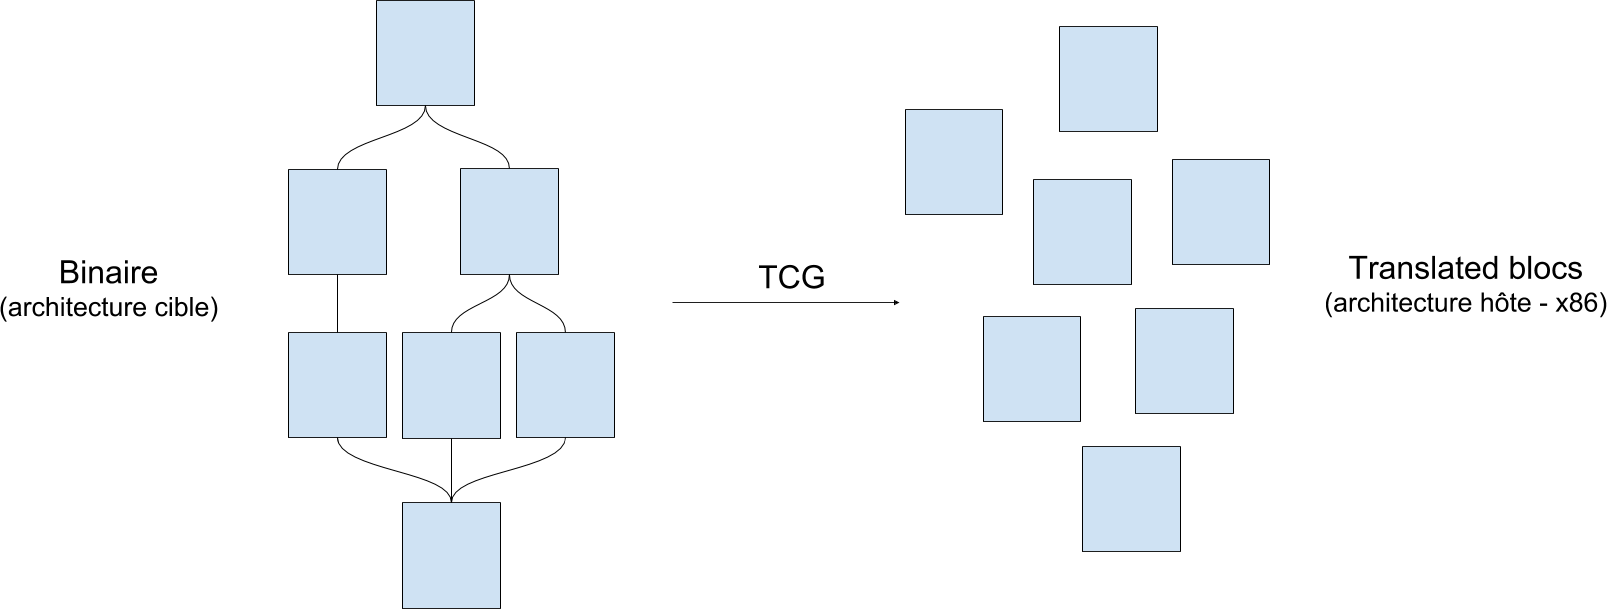
\includegraphics[width=.9\textwidth,height=.4\textheight]{../medias/qemu.png}
  \end{figure}

  \begin{itemize}
  \item cache les blocs traduits (Translated Blocs)
  \item intercepte les appels systèmes pour les transmettre au noyau de l'hôte
  \end{itemize}
\end{frame}

\begin{frame}[fragile]{Binaires quelconques et ciblant d'autres plateformes}{AFL avec le mode QEMU}
  \begin{itemize}
  \item version patchée de QEMU
  \item instrumentation "dynamique" des blocs traduits
  \end{itemize}

  \begin{lstlisting}[language=C]
    if (block_address > elf_text_start
        && block_address < elf_text_end) {
      cur_location = (block_address >> 4) ^ (block_address << 8);
      shared_mem[cur_location ^ prev_location]++;
      prev_location = cur_location >> 1;
    }
  \end{lstlisting}

  \begin{itemize}
  \item "fork server" et cache des blocs traduits partagé
  \item deux à cinq fois plus lent
  \end{itemize}
\end{frame}

\begin{frame}{Binaires quelconques et ciblant d'autres plateformes}{Autres versions d'AFL}
  \begin{block}{android-afl (*nix system)}
    \begin{itemize}
    \item adapter \lstinline{afl-gcc} pour cibler l'architecture ARM
    \item adapter \lstinline{afl-as} pour injecter de l'ARMv7
    \item remplacer \lstinline{sys/shm.h} (non disponible sous Android)
    \end{itemize}
  \end{block}

  \begin{exampleblock}{WinAFL (ProjectZero)}
    \begin{itemize}
    \item \sout{instrumentation}, \sout{fork server}
    \item instrumentation dynamique avec \lstinline{DynamoRIO}
    \end{itemize}
  \end{exampleblock}
\end{frame}
